 \subsection{Electronic chain linearity}

In order to prepare the data acquistion system, the entire electronical chain
was tested beforehand. In fact it is crucial that the response of each
electronic device used behaves linearly, as the information about the energy
of the incident particle must be univocally extracted at the end of the chain.

\begin{figure}[h]
  \centering
  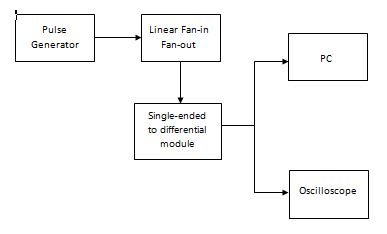
\includegraphics[scale=.5]{img/electronic_chain_diagram.JPG}
  \caption{The electronic chain}
  \label{chain}
\end{figure}

The setup used is shown in Fig.~\ref{chain}. The output of a pulse generator (\num{100}ns square pulse of variable amplitude) is fed into a Fan-in Fan-out which reproduces the same signal for 12 channels, this signals are given in input to a single-ended to differential amplifier custom board, in order to do this a cable was made.
The output of the board as seen from the oscilloscope is shown in Fig.~\ref{osc}. The shape of the rising edge of this signal will be sampled during the acquisition from the detector in order to perform PSA on each event.


\begin{figure}[h]
  \centering
  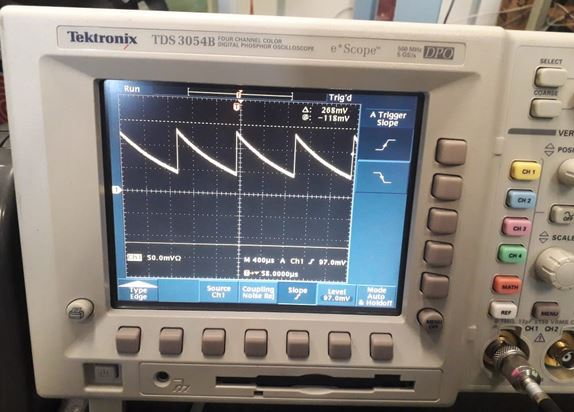
\includegraphics[scale=.35]{img/test_signal_oscilloscope.JPG}
  \caption{The output signal from the differential amplifier board, as seen on the oscilloscope.}
  \label{osc}
\end{figure}

From the board the signal is given to a 100 MHz 14-bit resolution digitizer throught a MDR-26 connector
At the signal is the applied, with an FPGA, a trapezoidal filter with its charateristics \emph{risetime} and \emph{flat top} width parameters (Moving Windows Analysis)~\cite{salathe}, this step is crucial because because the height of the peak from the differential amplifier board will be directly proportional to the energy of the incident particle in the detector.
The height trapezoidal filter with the right parameters then gives the information on the intensity of the peak available for longer time.


The output of the trapezoidal filter is then sampled throught the acquisition software that also control the MWA variables, the software records the amplitude of the output and saves it into different channels during the time of the acquisition. Histogram are then saved at the end, the software TKT is used to perform the fit on the peak obtained for the different pulse amplitude. 

The linearity of the response of the boards is evalueted fitting the data and checking the residuals plot as in Fig.~\ref{calib:plot:1} for all the 24 channels on the board.

\begin{figure}[th]
  \centering
  \begin{minipage}[b]{0.45\textwidth}
    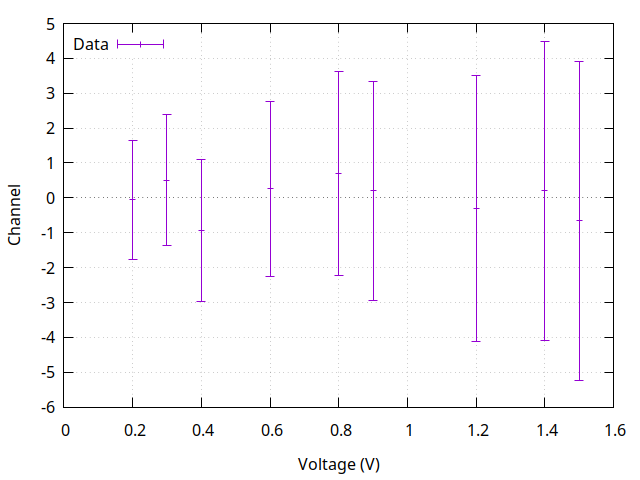
\includegraphics[width=\textwidth]{img/first_board_line/data_2/calib_1.png}
    \caption{Residual Plot for the the fit on the first channel on the tested board}
    \label{calib:plot:1}
  \end{minipage}
  \hfill
  \begin{minipage}[b]{0.45\textwidth}
  \begin{tabular}{lll}
    Voltage (V) & Channel & $\sigma$ \\
    \midrule
    0.2 & \num{393570.1} & 1.7 \\
    0.3 & \num{393753.2} & 1.8 \\
    0.4 & \num{393934.3} & 2.0 \\
    0.6 & \num{394300.5} & 2.5 \\
    0.8 & \num{394666.1} & 2.9 \\
    0.9 & \num{394848.1} & 3.1 \\
    1.2 & \num{395395.2} & 3.8 \\
    1.4 & \num{395760.8} & 4.3 \\
    1.5 & \num{395942.4} & 4.6 \\
    \bottomrule
  \end{tabular}
  \caption{Data for the fit}
  \label{calib:1}
  \end{minipage}
\end{figure}

All the channels gave fairly similar results, therefore confirming the linearity of the response of the electronic chain and an overral well behavior of the differential board tested.

\subsection{Testing the TRACE detector}

In order to test the TRACE detector along with its preamplifier, it was put in a vacuum chamber, with a $\alpha$-ray source (Fig.~\ref{trace_chamber}).


\begin{figure}[h]
  \centering
  \includegraphics[scale=.05]{img/trace_chamber.jpg}
  \caption{The TRACE detector inside the chamber along with its preamplifier boards and the alpha source.}
  \label{trace_chamber}
\end{figure}

To connect the integrated charge-sensitive pre-amplifiers to the TRACE silicon detector prototypes a custom board was designed and realized. Each board can host 2 ASIC pre-amplificators designed by INFN Milano and University of Milano with 8 channels each. The ASICS can be reconfigured using different soldering in order to accept the back channel. As each detectors is segmented in 60 pads of 4 $mm^2$, a total of 4 pre-amplification boards are required by telescope
The amplified signals is going out of the chamber via a flat cable connected to a FISCHER 27-pins connectors feedthrough making the bridge between the reaction chamber under vacuum ($10^{-3}$ mbar) and the laboratory. Outside of the chamber, from each FISCHER connector, the cables are divided in two 12-pins MOLEX connectors mounted on the Single-ended-to-differential modules. From here the signal goes directly to the 14-bits 100 MHz home made digitizer of the GALILEO array using MDR-26 connectors and 10 m cables.


The acquisition is triggered by the back portion of the detector (channel 0), and is performed as in the former section. The resolution is tested using the three peaks of the source (Tab.~\ref{peaks})

\begin{figure}[th]
  \centering
 \begin{tabular}{lc}
    Source & $E_\alpha$ (MeV)  \\ 
    \midrule
    \ce{^239Pu} & 5.1566  \\
    \ce{^241Am} & 5.4856  \\
    \ce{^244Cm} & 5.8048 \\
    \bottomrule
  \end{tabular}
  \caption{The predominant peaks from the triple-alpha source.}
  \label{peaks}
\end{figure}

\subsection{GALTRACE experiment}

The experiment was performed in July 2019 at the Legnaro National Laboratory
(Italy). A \ce{^13C} beam, with energy of $23$ MeV and intensity around $1$ pnA
was focused on a $0.1$ mg/cm thick \ce{^19 F} -\ce{^7 Li} -\ce{^12 C} target.
Two TRACE silicon detectors were placed inside the GALILEO HPGe array
scattering chamber. A common electrode covered the entire ohmic side of the
detector.

\bigbreak

Inside the chamber, the detectors were connected with a short cable to a
16-channel charge-sensitive preamplifier, designed at INFN Milano~\cite{strano}.
The preamplifier gain was $45$ mV/MeV yeilding a dynamic range of
approximately 100 MeV. The trigger of the acquisition was the signal from the
common electrode. The signals from one detector were sent to the digital
acquisition, while the second detector was connected to the analog read-out
line.

\bigbreak

The chain of the digital acquisition allowed to collect the signals (“traces”)
digitized by the 100 MHz sampling module. The length of the recorded trace was
1 $\mu$s, giving 100 points, at every 10 ns each. This length of the traces
was chosen to assure recording the full rise time on the one hand and at the
same time minimize the amount of written data. The signals were recorded,
digitized and afterwards processed to extract the relevant observables. The
placement of the TRACE module in the chamber with the ohmic side facing the
reaction products was important to enhance the PSA capability. The signals
were collected both from the ohmic side of the detector as well as from a few
groups of pads (or single pads).

\bigbreak

The trigger of the TRACE acquisition, obtained in this case from a digital
leading edge discriminator embedded in the module, was the signal from the
common electrode (“BACK”). The signals from the pads were collected only if
the BACK signal was present.